\subsection{MCRP Hardware Performance Evaluation}
\label{MCRPhardware}

Experiments are also implemented on hardware in realistic environments.  The hardware is tested in both home and office environments since~\cite{homearea} suggests that the two are drastically different.  The same experimental set up is tried in each environment.  The test network consists of 10 nodes; 1 border router and 9 duty cycled nodes.  At the highest power level nodes have a range of approximately 25 metres.  In indoor experiments this would mean that most nodes were in direct communication.  To change this we set the power level to -40dB relative to maximum giving a range of 15-80 cm (depending on intervening interference).  At this power level not all nodes are in direct communication but the positions were selected to allow each node to be in range of at least one other in order that a tree forms.  For the single channel protocol experiment each channel is measured for interference.  The protocol is tested on the channel with the lowest interference and the channel with the highest interference.

The first section of the experiment is "warm up" to allow for network formation.  This is forty five minutes for MCRP to complete set up and channel changes. During the experiment period four hundred and fifty packets are sent in total, fifty from each node at a rate of one per minute.  Each experiment is repeated ten times.  End-to-end packet delivery is used as the performance metric.  Unlike in the emulation results, the RPL tree formation set up is affected by the interference during initialisation. The network could be formed differently at each iteration.  

Nodes with direct connection to the LPBR must send on the LPBR listening channel and hence do not benefit from multi-channel.  However, several nodes were able to run MCRP processes. The tree topology formed differently each time depending on the radio coverage and interference level which affect the RPL ETX value for next hop selection. By increasing the number of nodes and area coverage, it increases the chances that the nodes would have routes to or from which enables MCRP to be executed.  

\begin{figure}
\centering
\subfigure[Residential environment]
{\label{fig:hardwareHome}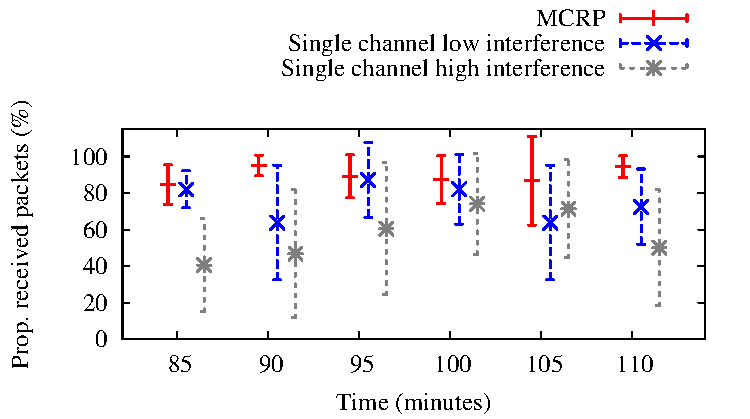
\includegraphics[width=0.45\textwidth]{figures/home.pdf}}
\subfigure[Office environment (UCL)]
{\label{fig:hardwareUCL}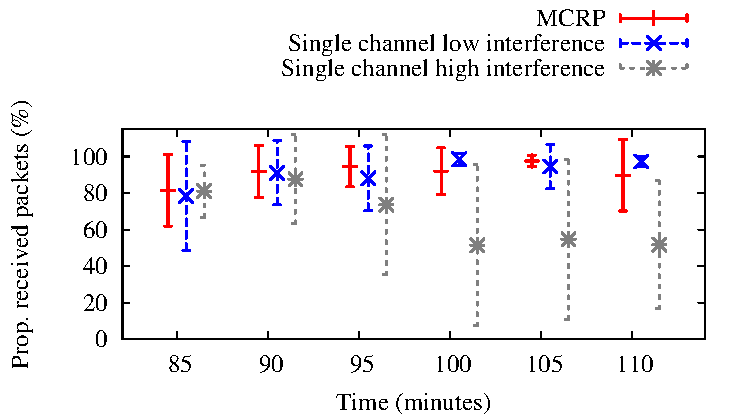
\includegraphics[width=0.45\textwidth]{figures/ucl.pdf}}
\caption{Real world: Level of packet loss for MCRP and single channel}
\label{fig:hardware}
\end{figure}

Figure \ref{fig:hardware} show the results from the experiment in residential and office environments for MCRP compared to the single channel protocol results for the channel with lowest interference and the channel with highest interference.  It can be clearly seen that in all experiments the error bars are high indicating that performance is extremely variable between runs of the experiment.  The MCRP protocol had higher mean packets received than the single channel protocol with high interference and comparable mean with the single channel protocol with low interference.  The MCRP protocol tended to have lower variance in performance particularly in the residential environment.  This demonstration shows that MCRP works on real hardware in realistic settings.  There was little demonstrated performance gain, possibly because of the small number of nodes used but MCRP did have more consistent performance in terms of packets received.
